\chapter{Podstawy teoretyczne}
Jak wspomniano w rozdziale~\ref{sec:cele}, dane wejściowe dla programu są wskazaniami pomiarów z~poszczególnych posterunków opadowych. Są to dane punktowe, zatem aby oszacować ilość wody jaka spadła na zadanym obszarze konieczne jest przeprowadzenie ich przekształcenia w~celu wyznaczenia opadu powierzchniowego.

\section{Powszechne metody wyznaczania opadu powierzchniowego}

Istnieje wiele metod wyznaczania średniego opadu powierzchniowego. Począwszy od prostego obliczenia średniej arytmetycznej wartości z~posterunków opadowych, poprzez metody wieloboków, izohiet po hipsometryczną. Różnią się one dokładnością, sposobem aproksymacji czy też poziomem zaawansowania. Każda jest też dostosowana do odpowiednich warunków analizowanego terenu. Poniżej znajduje się ich krótkie przybliżenie~\cite{obliczanie_opadu_sredniego, metody_obliczania_pb, opad_metody}.

\subsection{Metoda Thiessena}
Zwana także metodą wieloboków lub wielokątów równego zadeszczenia. Preferowana w~przypadku terenów nizinnych o~niewielkim zróżnicowaniu rzeźby. Walorem dla jej zastosowania jest równomierne rozmieszczenie posterunków opadowych. Stosuje się tu triangulację, a~następnie wyznaczając symetralne boków powstałych trójkątów tworzy się wieloboki, które odpowiadają poszczególnym posterunkom opadowym. Wskazanie posterunku przypisywane jest do wieloboku i~mnożone przez jego powierzchnię (uwzględniając granice zlewni). Sumując te iloczyny otrzymuje się oczekiwane wskazanie opadu powierzchniowego.

\begin{figure}[!ht]
	\begin{subfigure}{.5\textwidth}
		\centering
		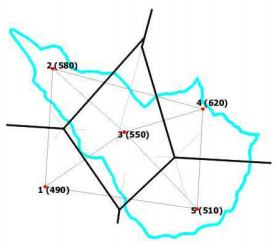
\includegraphics[width=0.7\linewidth]{thiessen1}
		\caption{Triangulacja i~symetralne boków.}
	\end{subfigure}%
	\begin{subfigure}{.5\textwidth}
		\centering
		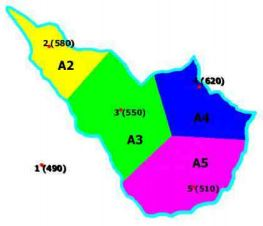
\includegraphics[width=0.7\linewidth]{thiessen2}
		\caption{Wieloboki wyznaczone na obszarze zlewni.}
	\end{subfigure}	
\caption{Schemat dla metody Thiesse. }
\end{figure}

\subsection{Metoda izohiet}
Metoda ta jest polecana dla analizy obszarów górskich, albowiem uwzględnia zależność między wysokością nad poziomem morza, a~wysokością opadu. Uznawana jest również za najbardziej dokładną.

Polega na podziale obszaru zlewni na fragmenty ograniczane przez kolejne izohiety. Dla każdego z~nich przyjmuje się wartość opadu będącą średnią arytmetyczną opadu na wyznaczających dany fragment izohietach. Taką samą zasadę stosuje się gdy granica zlewni przebiega blisko kolejnej izohiety. Jeżeli odległość ta jest znaczna, przyjmuje się wysokość opadu bliższej izohiety. Suma iloczynów wartości opadu i~powierzchni poszczególnych fragmentów stanowi wartość opadu na zadanej powierzchni.


\subsection{Metoda krzywej hipsometrycznej}
Podobnie jak metoda izohiet, zalecana jest dla badania terenów górskich, a~przede wszystkim małych zlewni. Jest stosunkowo pracochłonna, aczkolwiek dokładna.

W IV ćwiartce układu współrzędnych kreślona jest krzywa hipsometryczna oparta na mapie wysokościowej zlewni. Obrazuje ona zależność wysokości nad poziom morza (oś $X$) i~powierzchni zlewni (oś $Y$). Linia w~ćwiartce II nazywana jest krzywą gradientową opadów atmosferycznych. Jest to korelacja wzniesienia posterunku opadowego na osi odciętych oraz wysokości zmierzonego opadu na osi rzędnych.

Dokonując rzutowania krzywej hipsometrycznej poprzez ćwiartkę III i II (w~oparciu o~krzywą gradientową) na ćwiartkę I wyznaczana jest kolejna krzywa (zwana pluwiometryczną). Pole obszaru znajdującego się pod nią to rozmiar opadu na analizowanym obszarze. Opisany proces obrazuje rysunek~\ref{fig:hipsometryczna}.

\begin{figure}[!ht]
\centering
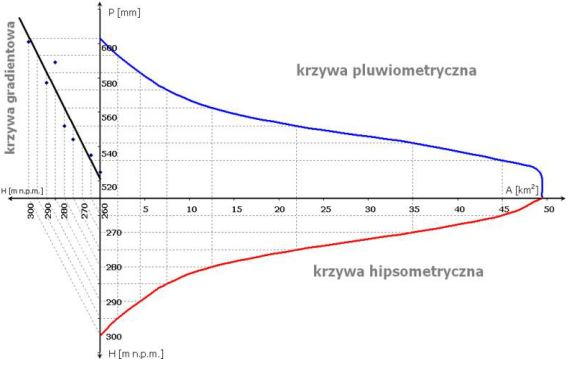
\includegraphics[width=0.7\linewidth]{hipsometryczna}
\caption{Wykres metody hipsometrycznej.}
\label{fig:hipsometryczna}
\end{figure}

\subsection{Metoda regionów opadowych}
Analizując zlewnię pod kątem cech fizyczno-geograficznych wydziela się obszary o~podobnych warunkach pogodowych. Wskazanie opadu na każdym z~nich stanowi średnia arytmetyczna pomiarów z~posterunków opadowych znajdujących się wewnątrz niego. Uwzględniając ograniczenie granicami zlewni wylicza się powierzchnię poszczególnych fragmentów i~mnoży ją przez wskazanie opadu. Podobnie jak w~innych metodach - suma takich iloczynów stanowi wielkość opadu w~zlewni.

Metoda ta jest mniej dokładna. Naturalnie, spisuje się najlepiej gdy obszar zlewni jak najbardziej pokrywa się z~wyznaczonymi regionami. Jej atutem jest niewielki poziom skomplikowania.

\begin{figure}[!ht]
\centering
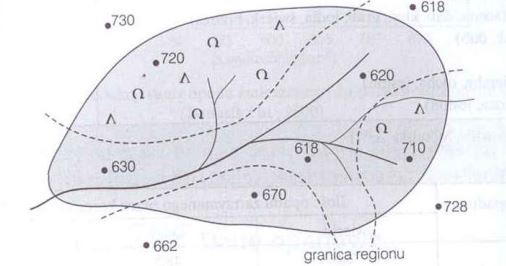
\includegraphics[width=0.5\linewidth]{regiony_opadowe}
\caption{Schemat regionów opadowych (źródło:~\cite{metody_obliczania_pb}).}
\label{fig:regiony_opadowe}
\end{figure}


\section{Zastosowana metoda}
\label{sec:zastosowana_metoda}
Jak wspomniano we wstępie, praca ta traktuje o analizie danych pojedynczego opadu, a~nie zbieranych przez pewien okres czasu. Przy wyborze sposobu przekształcenia danych jest to bardzo istotne kryterium, które wraz z~możliwością jak najlepszego dopasowania do kształtu zlewni stanowiło główne wymagania tej części pracy. Brano także pod uwagę poziom skomplikowania implementacji stosowanego rozwiązania. Wybór padł na połączenie techniki triangulacji wraz z~interpolacją przy użyciu płaszczyzny.

\begin{figure}[!ht]
	\centering
	\includegraphics[scale=0.7]{algorytm}
	\caption{Schemat krokowy zastosowanej metody}
	\label{fig:algorytm}
\end{figure}

%Triangulacja polega na stworzeniu siatki trójkątów o~wierzchołkach w~zadanych punktach (w tym wypadku są to posterunki opadowe o znanej wysokości opadu). 
Zastosowano algorytm triangulacji Delaunay'a, który wprowadza dodatkowe ograniczenie na tworzone trójkąty. Mianowicie, okrąg opisany na każdym z~nich nie może zawierać innych punktów siatki poza wierzchołkami danego trójkąta. Ta metoda ma na celu maksymalizację równoboczności powstałych trójkątów, a~co za tym idzie, równomierność budowanej siatki.

\begin{figure}[!ht]
	\centering
	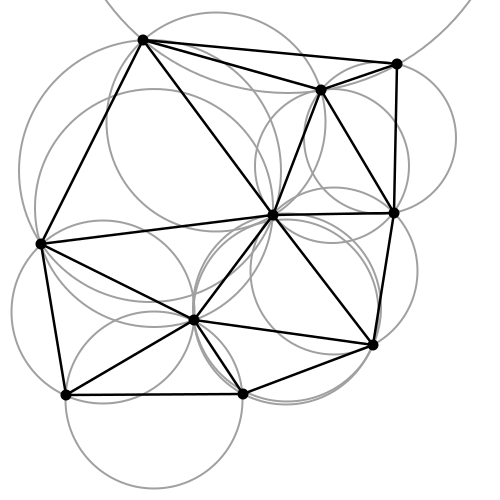
\includegraphics[scale=0.3]{delaunay}
	\caption{Schemat realizacji warunku Delaunay'a (źródło: \textit{www.wikipedia.pl}).}
	\label{fig:delaunay}
\end{figure}

Po zastosowaniu triangulacji, następnym etapem jest wyznaczenie punktów, dla których należy interpolować wartość opadu. Tymi punktami są poszczególne węzły granicy wskazanej zlewni oraz miejsca przecięcia tej granicy z~krawędziami trójkątów. Wraz z~posterunkami opadowymi znajdującymi się wewnątrz obszaru dla jakiego wyznaczany jest opad powierzchniowy będą stanowiły węzły kolejnej triangulacji.

Wyznaczenie wartości dla wskazanych punktów odbywa się poprzez interpolację płaszczyzną przechodzącą przez trzy punkty (będące wierzchołkami kolejnych trójkątów). Ustalane są współrzędne wektorów normalnych dla poszczególnych płaszczyzn (czyli wektorów prostopadłych do powierzchni danej płaszczyzny), a~następnie korzystając ze wzoru~\ref{eq:wartosc_interpolowana}, wyznaczana jest wartość opadu ($z$) w~punkcie o~zadanych współrzędnych~$x$~i~$y$.

Równanie płaszczyzny przedstawia się następująco.

\begin{equation}
\begin{gathered}
A(x - x_0) + B(y - y_0) + C(z - z_0) = 0 \\
[A, B, C] = (P_2 - P_1) \times (P_3 - P_2)
\label{eq:rownanie_plaszczyzny}
\end{gathered}
\end{equation}
gdzie
% eqwhere z aghdpl powoduje błąd
\begin{description}[leftmargin=3cm, itemsep=0cm, labelsep=0cm]
	\item[$x_0, y_0, z_0$] współrzędne punktu należącego do płaszczyzny,
	\item[{[}$A, B, C${]}] wektor normalny płaszczyzny, %rozwiązać problem z [ ] jako wektor
	\item[$A, B, C$] nie mogą być jednocześnie równe 0.
\end{description}
%
Co po przekształceniu daje
\begin{equation}
\label{eq:wartosc_interpolowana}
	z = \frac{A(x - x_0) + B(y - y_0)}{-C} + z_0
\end{equation}
gdzie $C \neq 0$.


Jeżeli $C$, ze wzoru~\ref{eq:wartosc_interpolowana}, przyjmuje wartość 0 oznacza to, iż w~każdym wierzchołku trójkąta opad był zerowy. Wówczas punktowi interpolowanemu przypisuje się takowe wskazanie.

Po przeprowadzeniu interpolacji wartości dokonuje się ponownej triangulacja, tym razem z~użyciem punktów interpolowanych oraz posterunków wewnątrz zlewni. Nowopowstała siatka trójkątów, wraz z~trzecim wymiarem jakim jest wysokość opadu, tworzy zbiór brył o~trójkątnych podstawach. Wyznaczając i~sumując objętość opadu w~każdej z~nich uzyskiwany jest łączny opad na wskazanej zlewni~\cite{matematyka_poradnik, mathMonthly}.

\begin{equation}
	V = \sum_{i=1}^{n}P_{pi}*\frac{h_{i1}+h_{i2}+h_{i3}}{3}
\label{eq:opad_powierzchniowy}
\end{equation}
gdzie
\begin{description}[leftmargin=3cm, itemsep=0cm, labelsep=0cm]
	\item[$V$] łączna objętość opadu,
	\item[$n$] ilość wyznaczonych brył,
	\item[$P_{pi}$] pole podstawy $i$-tej bryły,
	\item[$h_{i1}, h_{i2}, h_{i3}$] długość krawędzi bocznej $i$-tej bryły (wartość opadu) w~danym wierzchołku.
\end{description}




\section{Możliwe rozszerzenia algorytmu}
Oczywiście można dążyć do usprawnienia metody przekształcania danych wejściowych.
Przykładowe rozszerzenia mogą obejmować
\begin{itemize}
\item{ Analizę sąsiednich dla trójkąta punktów i~na ich podstawie wyznaczenie wartości opadu w~środku zadanego fragmentu, a~dalej dzielenie go na mniejsze. }

\item{ Interpolację powierzchnią inną niż płaszczyzna. Kształt powierzchni definiować na bazie większej ilości punktów znanych. }

\item{ Uwzględnienie ukształtowania terenu podczas analizy obszaru zlewni. }
\end{itemize}